In the previous chapter we toured loci phenomena for billiard 3-periodics. Here we continue this exploration for other for 3-periodic families in other concentric, axis-aligned ellipse pairs, shown in \cref{fig:06-six-caps}.

\begin{figure}
    \centering
    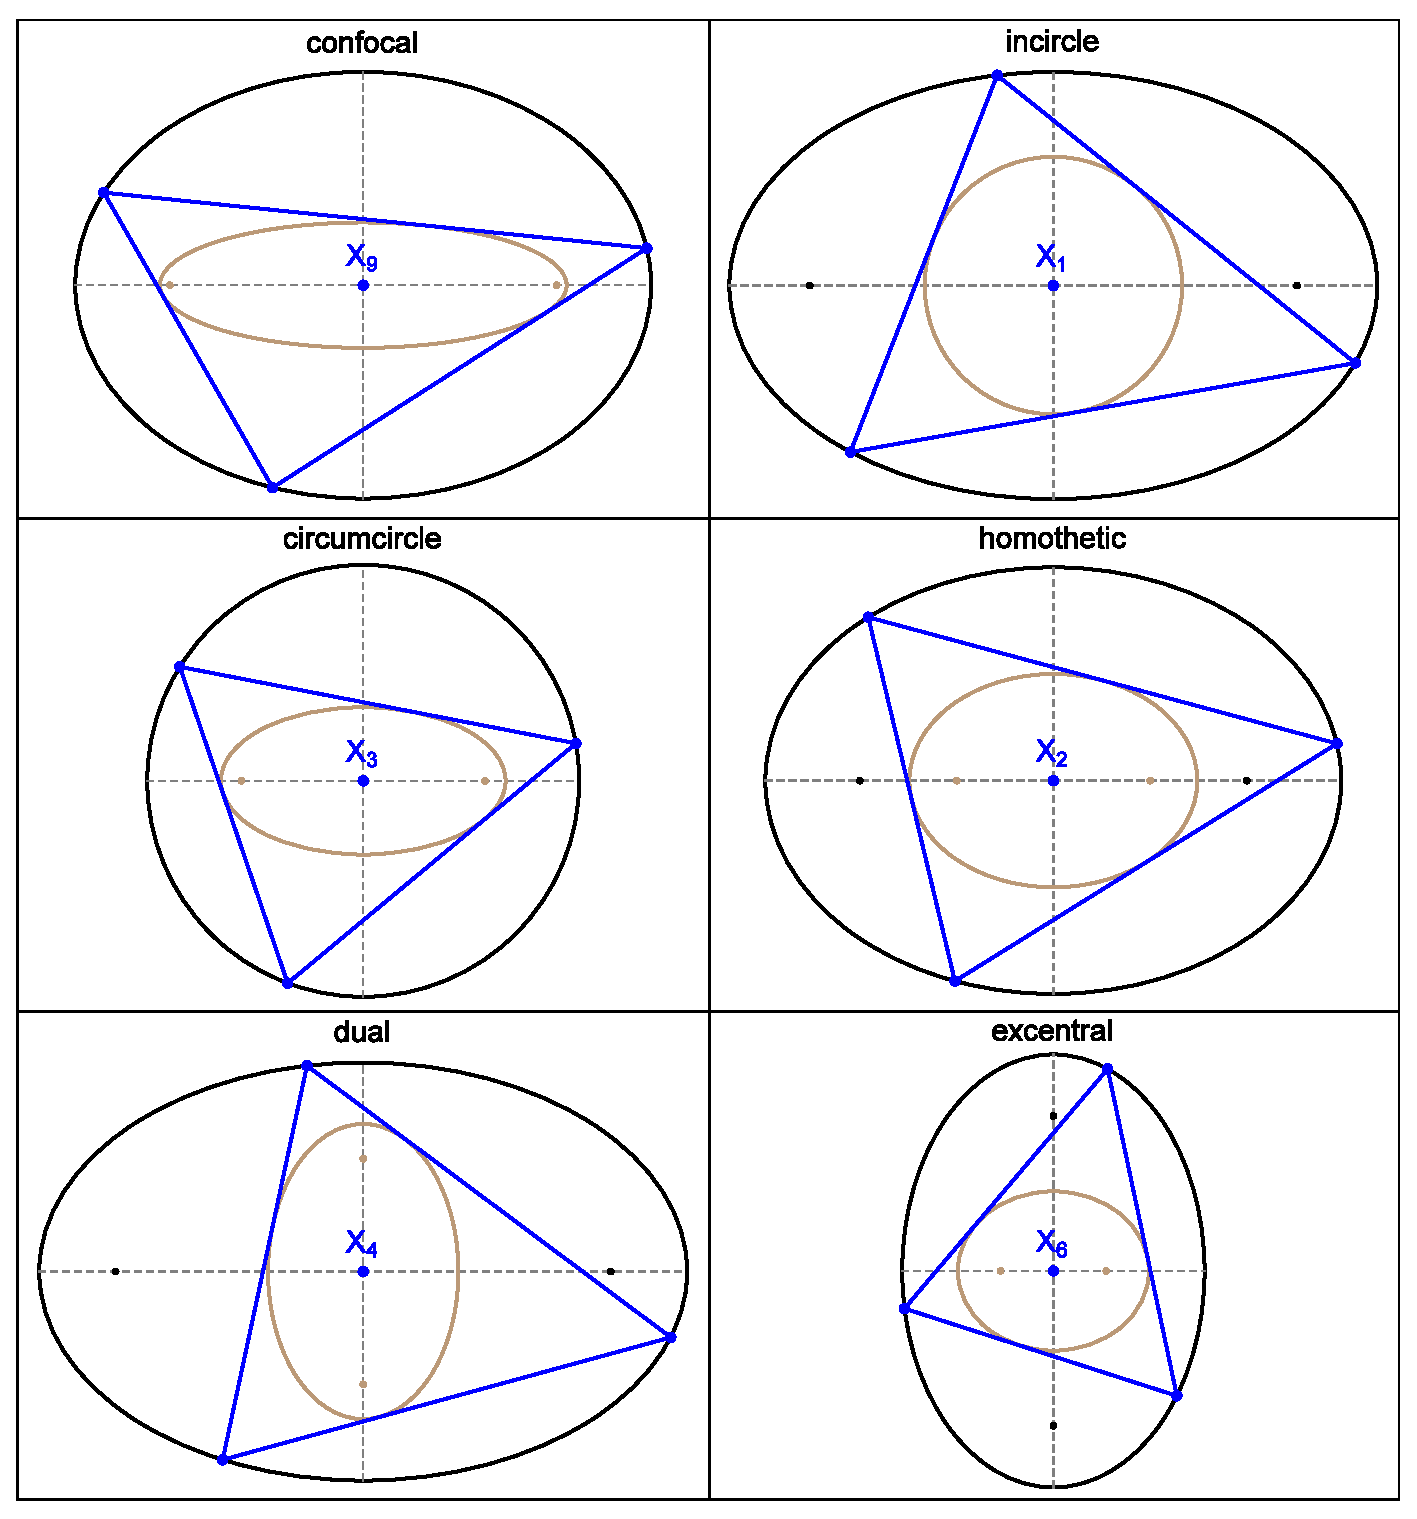
\includegraphics[width=\textwidth]{chap_06/pics/pics_06_015_six_caps_perp}
    \caption{The five concentric, axis-parallel (CAP) families whose loci are studied in this chapter. The confocal family is treated in \cref{chap:05-confocal-loci}. \href{https://youtu.be/14TQ5WlZxUw}{Video}}
    \label{fig:06-six-caps}
\end{figure}

Recall Cayley's condition for a CAP pair to admit a Poncelet 3-periodic family: $a_c/a+b_c/b=1$, where $a>b>0$, $a_c>0$, and $b_c>0$.

